\documentclass{beamer}
%
% Choose how your presentation looks.
%
% For more themes, color themes and font themes, see:
% http://deic.uab.es/~iblanes/beamer_gallery/index_by_theme.html
%
\mode<presentation>
{
 \usetheme{Hannover}    % or try Darmstadt, Madrid, Warsaw, ...
  \usecolortheme{edinburgh} % or try albatross, beaver, crane, ...
  \usefonttheme{default}  % or try serif, structurebold, ...
  \setbeamertemplate{navigation symbols}{}
  \setbeamertemplate{caption}[numbered]
} 

\usepackage[english]{babel}
\usepackage[utf8x]{inputenc}
\usepackage{float}
\usepackage{tipa}
\usepackage{multimedia}
\usepackage{epstopdf}
\usepackage{tikz}
\usepackage{hyperref}
\usepackage{listings}
\title[Semisynthetic Speech Stimuli for Sociophonetic Experiments]{Generating natural-sounding semisynthetic speech stimuli for sociophonetic experiments}
\institute{Daniel Lawrence\\School of Philosophy, Psychology \& Language Sciences\\The University of Edinburgh}
\date{dlawrenc$@$staffmail.ed.ac.uk\\$@$danielplawrence}
\begin{document}
\lstset{ %
  backgroundcolor=\color{white}, 
  basicstyle=\footnotesize,       
  breakatwhitespace=false,        
  breaklines=true,                 
  captionpos=b,                    
  commentstyle=\color{green},   
  escapeinside={\%*}{*)},        
  extendedchars=true,              
  frame=single,                  
  keywordstyle=\color{blue},       
  language=Prolog,                
  numbers=left,                    
  numbersep=5pt,                   
  numberstyle=\tiny\color{gray},
  rulecolor=\color{black},        
  showspaces=false,               
  showstringspaces=false,          
  showtabs=false,                  
  stepnumber=2,                    
  stringstyle=\color{blue},   
  tabsize=2,                      
  title=\lstname,                  
  morekeywords={not,\},\{,preconditions,effects },            
  deletekeywords={time}            
}
\begin{frame}
  \titlepage
\raggedleft 
\vspace*{-0.5cm}
\includegraphics[scale=0.35,keepaspectratio]{JPG_RGB_Large.jpg}

\raggedright
\vspace*{-1.25cm}
\includegraphics[scale=0.225,keepaspectratio]{2Line2ColCMYK_CS3.eps}


\end{frame}

% Uncomment these lines for an automatically generated outline.
%\begin{frame}{Outline}
%\tableofcontents


%\end{frame}

\section{Introduction}
\begin{frame}{Introduction}
A typical aim of a sociophonetic perception study is to explore the impact of a single variable on a social judgment. 
Options:
\begin{itemize}
\item{Use phonetically diverse natural stimuli (e.g. Clopper \& Pisoni, 2004)}
\item{Use stimuli performed by variable speakers (e.g. Evans \& Iverson, 2004)}
\item{Use stimuli performed by phoneticians (e.g. Kubisz, 2014)}
\item{Use synthetic or semisynthetic stimuli (e.g. Kendall \& Fridland, 2012; Hay, Warren \& Drager, 2006)}
\end{itemize}
\end{frame}
\section{Parametric synthesis}
\begin{frame}{Parametric synthesis}
Basic source-filter theory (Fant, 1960):
\begin{itemize}
\item{Treat the speech signal as a combination of a sound source and vocal tract resonances, plus the effect of radiation from the lips:}
\end{itemize}
\hspace{-0.5cm}
\includegraphics[scale=0.6,keepaspectratio]{fant.png}
\end{frame}
\begin{frame}{Parametric synthesis}
Basic source-filter theory (Fant, 1960):
\begin{itemize}
\item{Treat the speech signal as a combination of a sound source and vocal tract resonances, plus the effect of radiation from the lips:}
\end{itemize}
\includegraphics[scale=0.225,keepaspectratio]{aa_source.pdf}
\includegraphics[scale=0.225,keepaspectratio]{aa_filter.pdf}
\includegraphics[scale=0.225,keepaspectratio]{aa_conv.pdf}
\begin{itemize}
\item{To synthesize speech, we need to generate an excitation source and pass it through a set of digital filters}
\end{itemize}
\end{frame}
\begin{frame}{Parametric synthesis}
Parametric synthesis:
\begin{itemize}
\item{Basic schematic of the Klatt (1980) synthesizer}
\end{itemize}
\includegraphics[scale=0.5,keepaspectratio]{klatt.png}
\end{frame}
\begin{frame}{Parametric synthesis}
Parametric synthesis:
\begin{itemize}
\item{Cascade branch of the Klatt (1980) synthesizer}
\end{itemize}
\includegraphics[scale=0.4,keepaspectratio]{cascade.png}
\begin{itemize}
\item{Each filter boosts the frequencies to match the resonances it represents.}
\end{itemize}
\end{frame}
\begin{frame}{Parametric synthesis}
In practice:
\begin{itemize}
\item{Specify parameters for every time point.}
\includegraphics[scale=0.4,keepaspectratio]{klatt_param.png}
\end{itemize}
\end{frame}
\begin{frame}{Parametric synthesis}
\begin{figure}
\includegraphics[scale=0.3,keepaspectratio]{coffee_klatt.pdf}
\end{figure}
\centering
\movie[start=5s, inlinesound]{\fbox{Play}}{coffee.wav}
\end{frame}
\begin{frame}[fragile]{Parametric synthesis}
Parametric synthesis in Praat:
\begin{itemize}
\item{Praat implements the Klatt synthesizer through `KlattGrid' objects}
\item{You can imagine these as 2D grids with time on the X-axis and the Klatt settings on the Y-axis}
\item{http://www.fon.hum.uva.nl/praat/manual/KlattGrid.html}
\end{itemize}
\begin{lstlisting}
#Create a KlattGrid
Create KlattGrid... aa 0 0.5 6 1 1 6 1 1 1
\end{lstlisting}
\end{frame}
\begin{frame}[fragile]{Parametric synthesis}
Parametric synthesis in Praat:
\begin{lstlisting}
#Add voicing amplitude, vowel formants, and pitch targets
Add voicing amplitude point... 0.0 0
Add voicing amplitude point... 0.04 90
Add voicing amplitude point... 0.25 90
Add voicing amplitude point... 0.5 90
Add pitch point... 0.0 150
Add pitch point... 0.5 150
\end{lstlisting}
\end{frame}
\begin{frame}[fragile]{Parametric synthesis}
Parametric synthesis in Praat:
\begin{lstlisting}
Add oral formant frequency point... 1 0.1 750
Add oral formant bandwidth point... 1 0.1 70
Add oral formant frequency point... 2 0.1 1250
Add oral formant bandwidth point... 2 0.1 120
Add oral formant frequency point... 3 0.1 2500
Add oral formant bandwidth point... 3 0.1 200
Add oral formant frequency point... 4 0.1 3900
Add oral formant bandwidth point... 4 0.1 300
#Synthesis
Play
To Sound
\end{lstlisting}
\begin{itemize}
\item{Can you modify the code to generate a high front vowel?}
\item{What about a diphthong?}
\item{Try running `klatt\_cardinal.psc'}
\end{itemize}
\end{frame}
\begin{frame}{Parametric synthesis}
Pros of fully-parametric synthesis:
\begin{itemize}
\item{Fine-grained control over parameters}
\item{Given unlimited time and accurate measurements of the parameters of a source item, in principle possible to synthesize any speech sound}
\item{Stimuli fully replicable as long as parameters are published}
\end{itemize}
\end{frame}
\begin{frame}{Parametric synthesis}
Cons of fully-parametric synthesis:
\begin{itemize}
\item{Properties of the glottal source particularly difficult to imitate.}
\item{This means that tokens often have a `robotic' quality -- perhaps not appropriate for some sociophonetic applications.}
\item{Parameter-setting can be very time consuming, particularly if we want to model dynamic properties of vowels.}
\end{itemize}
\end{frame}
\section{LPC-based methods}
\begin{frame}{LPC inverse-filtering}
An alternative: LPC inverse-filtering
\begin{itemize}
\item{This technique has been implemented in a number of sociophonetic studies -- as far back as Graff, Labov \& Harris, 1984.}
\item{Detailed technical outline in Alku et al. 1999}
\item{This is what Bartek Plichta's \textit{Akustyk} does...}
\item{...although I don't know the details of how BP has implemented it.}
\end{itemize}
\end{frame}
\begin{frame}
Linear Predictive Coding
\begin{itemize}
\item{A technique for estimating the spectral envelope of a time-varying speech signal.}
\item{Origins in early television encoding -- black and white TV images are 3D grids (x,y,brightness) which vary over time.}
\end{itemize}
\begin{figure}
\centering
\includegraphics[scale=0.05,keepaspectratio]{bw_tv.jpg}
\end{figure}
\begin{itemize}
\item{However, values do not vary randomly -- the brightness of any point is likely to be related to the adjacent points}
\end{itemize}
\end{frame}
\begin{frame}
Linear Predictive Coding
\begin{figure}
\centering
\includegraphics[scale=0.4,keepaspectratio]{linear_predictive_filter.png}
\end{figure}
\footnotesize{Image courtesy of Simon King}
\end{frame}
\begin{frame}
Linear Predictive Coding
\begin{figure}
\includegraphics[scale=0.5]{signal.png}
\end{figure}
\end{frame}
\begin{frame}
Linear Predictive Coding
\begin{figure}
\includegraphics[scale=0.5]{signal_windowed.png}
\end{figure}
\end{frame}
\begin{frame}
Linear Predictive Coding
\begin{figure}
\includegraphics[scale=0.5]{one_window.png}
\end{figure}
\end{frame}
\begin{frame}
Linear Predictive Coding
\begin{figure}
\includegraphics[scale=0.5]{target_sample.png}
\end{figure}
\end{frame}
\begin{frame}
Linear Predictive Coding
\begin{figure}
\includegraphics[scale=0.5]{target_plus_coefs.png}
\end{figure}
\end{frame}
\begin{frame}
Linear Predictive Coding
\begin{figure}
\includegraphics[scale=0.5]{regression.png}
\end{figure}
\end{frame}
\begin{frame}
Linear Predictive Coding
\begin{figure}
\includegraphics[scale=0.5]{store_coefs.png}
\end{figure}
\end{frame}
\begin{frame}
Linear Predictive Coding
\begin{figure}
\includegraphics[scale=0.5]{bad_prediction.png}
\end{figure}
\end{frame}
\begin{frame}
Linear Predictive Coding
\begin{figure}
\includegraphics[scale=0.5]{error.png}
\end{figure}
\end{frame}
\begin{frame}
Linear Predictive Coding
\begin{figure}
\includegraphics[scale=0.5]{encoded_signal.png}
\end{figure}
\end{frame}
\begin{frame}
Linear Predictive Coding
\begin{figure}
\includegraphics[scale=0.5]{largest_errors.png}
\end{figure}
\end{frame}
\begin{frame}
Linear Predictive Coding
\begin{figure}
\includegraphics[scale=0.5]{signal.png}
\end{figure}
\end{frame}
\begin{frame}
Linear Predictive Coding
\begin{figure}
\includegraphics[scale=0.5]{smoothed_spectrum.png}
\end{figure}
\end{frame}
\begin{frame}
Linear Predictive Coding
\begin{itemize}
\item{Estimating the LPC filter is an optimization problem -- we find the best set of $a$ values for the given signal}
\item{The difference between the LPC model and the actual signal is the \textit{prediction residual} -- together, the estimated LPC filter and residual encode the entire signal:}
\end{itemize}
\centering{$e(n) = x(n) - \widehat{x}(n)$}
\begin{itemize}
\item{Because the largest errors tend to be around the largest changes in the signal, the residual approximates the pitch periods, `whitening' the signal by removing spectral characteristics.}
\end{itemize}
\end{frame}
\begin{frame}
\centering
\begin{figure}
\includegraphics[scale=0.9,keepaspectratio]{original_vowel.png}
\end{figure}
\begin{figure}
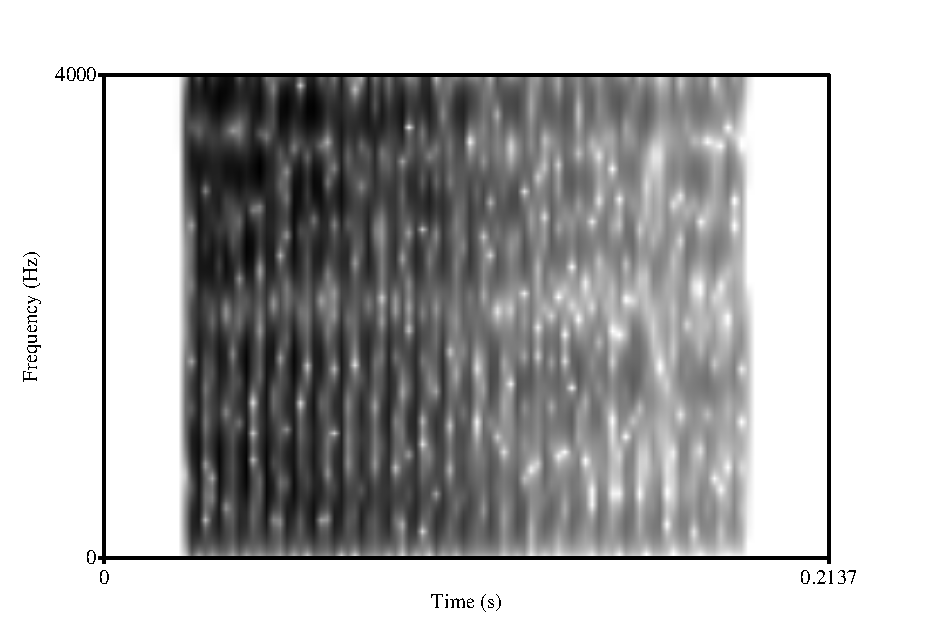
\includegraphics[scale=0.3,keepaspectratio]{source.eps}
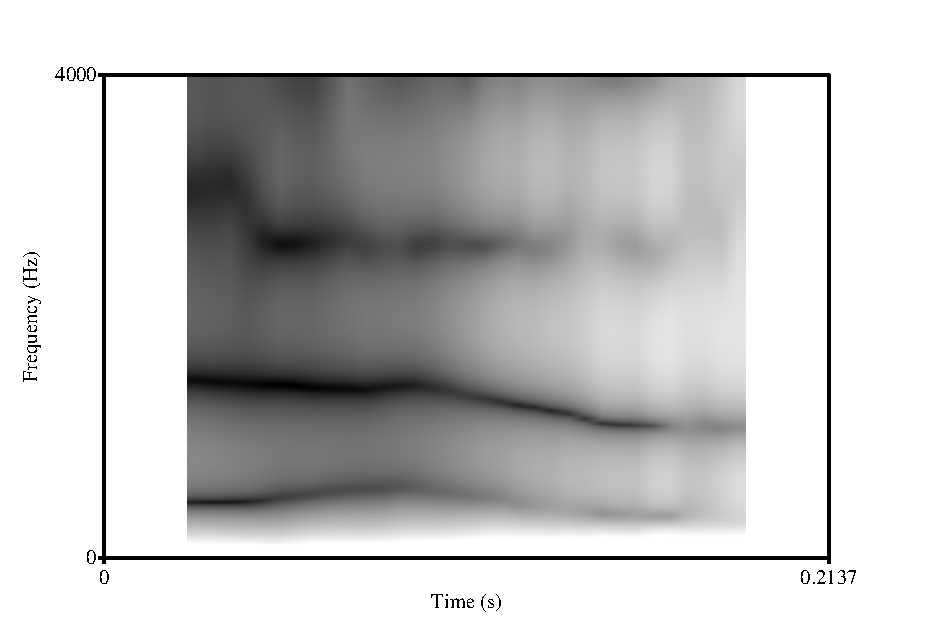
\includegraphics[scale=0.3,keepaspectratio]{LPC_filter.eps}
\end{figure}
\end{frame}
\begin{frame}
\begin{itemize}
\item{Now we can excite a digital filter bank with our natural source representation}
\end{itemize}
\begin{figure}
\includegraphics[scale=0.6,keepaspectratio]{LPC_synth.png}
\end{figure}
\end{frame}
\begin{frame}
\begin{itemize}
\item{Problem: LPC analysis results in the loss of the high-frequency component of the original sound}
\end{itemize}
\begin{figure}
\includegraphics[scale=0.5,keepaspectratio]{LPC_lossy.png}
\end{figure}
\movie[start=5s, inlinesound]{\fbox{Play}}{OF_no_HF.wav}
\end{frame}
\begin{frame}
\begin{itemize}
\item{Solution: Restore the HF component of the original sound after synthesis}
\end{itemize}
\begin{figure}
\includegraphics[scale=0.5,keepaspectratio]{synth_HF_added.png}
\end{figure}
\movie[start=5s, inlinesound]{\fbox{Play}}{synth_HF.wav}
\end{frame}
\begin{frame}
\begin{itemize}
\item{Problem: How can we ensure that we have a good source model?}
\end{itemize}
\begin{figure}
\includegraphics[scale=0.5,keepaspectratio]{not_very_white.png}
\end{figure}
\end{frame}
\begin{frame}
\begin{itemize}
\item{Solution: Following Alku (1992), filter iteratively, estimating spectral characteristics of glottal flow and vocal tract with different LPC orders}
\end{itemize}
\begin{figure}
\includegraphics[scale=0.4,keepaspectratio]{iaif_block.png}
\end{figure}
\end{frame}
\begin{frame}
\begin{itemize}
\item{Result: very high quality source-filter separation}
\end{itemize}
\begin{figure}
\includegraphics[scale=0.3,keepaspectratio]{not_very_white.png}
\includegraphics[scale=0.3,keepaspectratio]{much_more_white.png}
\end{figure}
\end{frame}
\begin{frame}
\begin{itemize}
\item{Finally, embed the vowel in a lexical item by splicing at zero-crossing points}
\end{itemize}
\begin{figure}
\includegraphics[scale=0.3,keepaspectratio]{concat.png}
\end{figure}
\end{frame}
\begin{frame}
\begin{itemize}
\item{End result:}
\end{itemize}
\begin{figure}
\includegraphics[scale=0.5,keepaspectratio]{final.png}
\movie[start=5s, inlinesound]{\fbox{Play}}{eight_step_goat.wav}
\end{figure}
\end{frame}
\begin{frame}{Complete process}
\end{frame}
\begin{frame}[fragile]{Resynthesis}
LPC inverse-filtering in Praat:
\begin{lstlisting}
#Estimate the LPC filter for a selected sound
#First we need to resample
Resample: 10000, 50
To LPC (burg): 8, 0.025, 0.005, 50
\end{lstlisting}
\end{frame}
\begin{frame}[fragile]{Resynthesis}
\begin{lstlisting}
#Take the inverse of this filter to get a representation of the source
selectObject: "Sound untitled_10000"
plusObject: "LPC untitled_10000"
Filter (inverse)
\end{lstlisting}
\end{frame}
\begin{frame}[fragile]{Resynthesis}
\begin{lstlisting}
#Generate a formant object and add 400 Hz to F2
selectObject: "LPC untitled_10000"
To Formant
selectObject: "Formant untitled_10000"
Formula (frequencies): "if row = 2 then self + 400 else self fi"
\end{lstlisting}
\end{frame}
\begin{frame}[fragile]{Resynthesis}
\begin{lstlisting}
#Combine the source and filter representations to make a new vowel
selectObject: "LPC untitled_10000"
selectObject: "Sound untitled_10000"
plusObject: "Formant untitled_10000"
Filter
Play
\end{lstlisting}
\begin{itemize}
\item{Try recording yourself producing a vowel (ctr+r). Select your vowel token and run `LPC\_cardinal\_iaif.praat'}
\end{itemize}
\end{frame}
\section{Summary}
\begin{frame}{Summary}
\begin{itemize}
\item{A range of options available when preparing perception experiments}
\item{Trade off between naturalness and control of phonetic detail}
\item{In some cases, the face validity of the experiment may be more important than others}
\item{In some cases, a lack of naturalness might even strengthen our arguments!}
\item{Importance of explicitness about manipulation methods: no black boxes}
\item{\textit{Praat} is capable of very sophisticated analysis and manipulations, and is open source}
\end{itemize}

\end{frame}
\section{References \& Links}
\begin{frame}{References}
\begin{itemize}
\footnotesize{
\item{Alku, P., Tiitinen, H., \& Naatanen, R. (1999). A method for generating natural-sounding speech stimuli for cognitive brain research. Clinical Neurophysiology, 110(8), 1329-1333.}
\item{Clopper, C. G., \& Pisoni, D. B. (2004). Some acoustic cues for the perceptual categorization of American English regional dialects. Journal of Phonetics, 32(1), 111-140.}
\item{Evans, B. G., \& Iverson, P. (2004). Vowel normalization for accent: An investigation of best exemplar locations in northern and southern British English sentences. The Journal of the Acoustical Society of America, 115(1), 352-361.}
\item{Hay, J., Nolan, A., \& Drager, K. (2006). From fush to feesh: Exemplar priming in speech perception. The linguistic review, 23(3), 351-379.}
\item{Klatt, D. H. (1980). Software for a cascade/parallel formant synthesizer. the Journal of the Acoustical Society of America, 67(3), 971-995.}
\item{Kubisz, A. (2014). The role of gendered sociolinguistic variants as perceptual cues. York Working Papers in Linguistics 1}
\item{Kendall, T., \& Fridland, V. (2012). Variation in perception and production of mid front vowels in the US Southern Vowel Shift. Journal of Phonetics, 40(2), 289-306.}}
\end{itemize}
\end{frame}
\begin{frame}{Links}
\begin{itemize}
\footnotesize
\item{Formant manipulation script on Github: https://github.com/danielplawrence/semisynthetic}
\item{Will Styler's resynthesis scripts: https://github.com\\/stylerw/styler\_praat\_scripts/tree/master/source\_filter\_vowel\_resynth}
\item{Similar stuff from Sam Kirkham: http://samkirkham.com/scripts/index.html}
\item{Instructions for source-filter synthesis in \textit{Praat}: http://www.fon.hum.uva.nl/praat/manual/Source-filter\_synthesis.html}
\item{PraatR: http://www.aaronalbin.com/praatr/}
\end{itemize}
\end{frame}
\end{document}
